\documentclass[12pt]{article}

\usepackage[english]{babel}
\usepackage[utf8]{inputenc}
\usepackage{fancyhdr}

\usepackage[margin=1in]{geometry}
\usepackage{pgf}
\usepackage{pgfplots}
\usepackage{siunitx}
\usepackage{tikz}
\usepackage{float}
\usepackage{amsmath}
\usepackage{enumitem}

\usepackage[font=small,labelfont=bf]{caption}
\usepackage{pstricks-add}
\usepackage{pgfplotstable}
\usepackage[nodisplayskipstretch]{setspace}

\usetikzlibrary{scopes}
\usetikzlibrary{angles,quotes}
\usetikzlibrary{calc}
\pgfplotsset{compat=1.5}
\graphicspath{ {/} }

\newcommand*{\I}{\imath}
\newcommand*{\J}{\jmath}
\newcommand{\norm}[1]{\lvert #1 \rvert}

\setlist[enumerate, 1]{label=\alph*.}

\begin{document}
\sisetup{per-mode=symbol}

\begin{titlepage}
    \begin{center}
        \vspace*{1cm}
        \textbf{Transients in an RC Circuit}

        \vspace{0.5cm}
        Lab: 06

        \vspace{1cm}

        \textbf{Jaden Moore}

        \vfill

        Orange Coast College\\
        Physics A280L\\
        April 26th, 2021

    \end{center}
\end{titlepage}

\pagestyle{fancy}
\fancyhf{}
\setlength{\headheight}{15pt}
\lhead{Transients in an RC Circuit}
\rhead{Lab: 06}
\cfoot{\thepage}

\section{Introduction}
In this lab, we use an oscilloscope to measure the voltage across a resistor that is connected in series to a charging capacitor. Consider a square wave released from a function generator connected to a circuit containing a $\SI{1}{\micro\farad}$ capacitor $C_1$ and a  $\SI{2000}{\ohm}$ resistor $R_1$. We then analyze the voltage across the resistor $R_1$ over time as the charge in the capacitor $C_1$ increases due to the square wave generator.

\section{Data and Analysis}
Below is a graph of the theoretical voltage through the resistor compared to the experimental voltage over time.

\begin{figure}[H]
    \begin{center}
        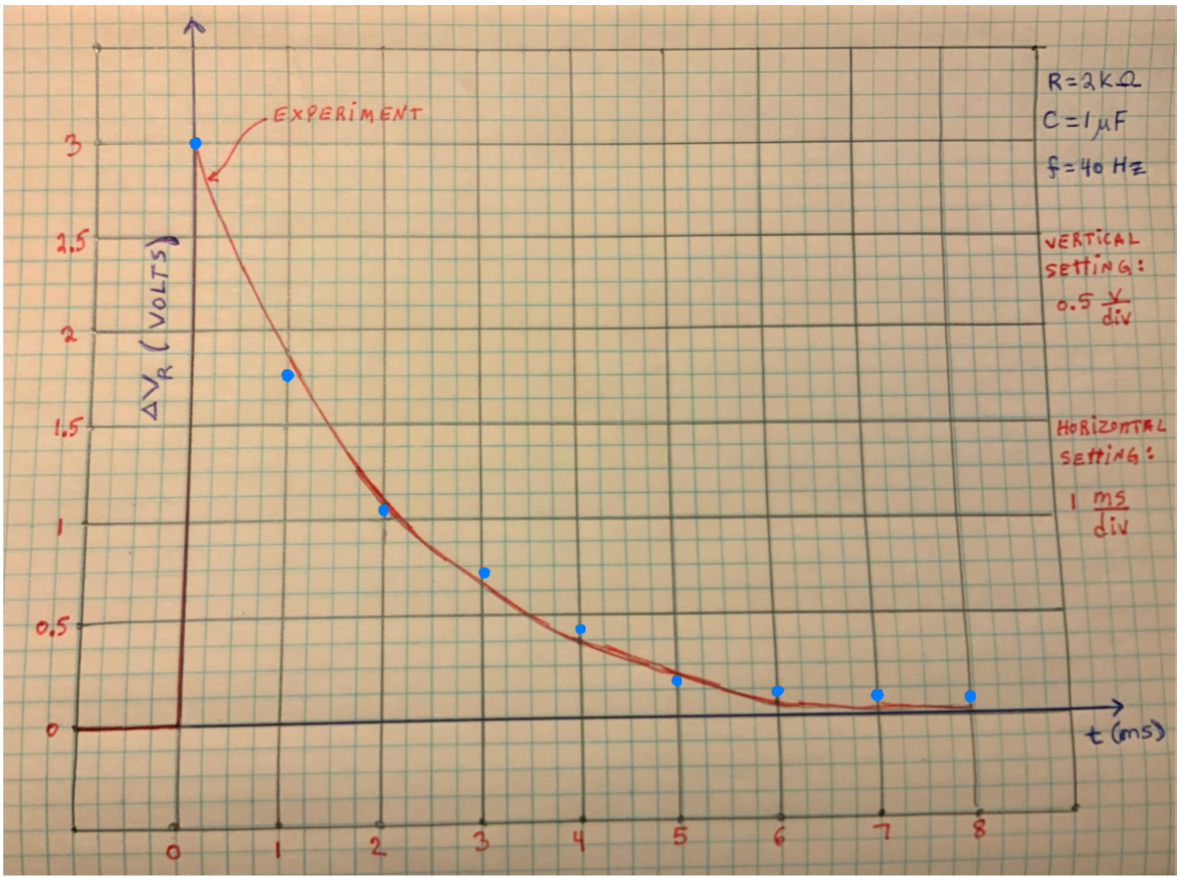
\includegraphics[scale=0.6]{Figure-1.png}
        \caption { Voltage across resistor over time}
    \end{center}
\end{figure}

A preliminary analysis of the graph indicates that as time increases, the voltage across the resistor decreases exponentially. This indicates that the capacitor is storing charge over time. From the lab, we get the equation for the theoretical voltage across the resistor to be:

\begin{equation} \label{1}
    \begin{split}
        \Delta V_R(t)=\varepsilon e^{-\frac{t}{RC}}
    \end{split}
\end{equation}

Where R is the resistance of the resistor, C is the capacitance of the capacitor $\varepsilon$ is the voltage of the square wave generator, and t is time. From the circuit, we get that $RC$ = 2 ms and $\varepsilon$ is 3 volts.

From this, we are able to calculate the theoretical voltage across the resistor. In the table below, we compare the experimental voltage obtained from the oscilloscope with the theoretical voltage over time. 

\newcolumntype{P}[1]{>{\centering\arraybackslash}p{#1}}

\setlength{\tabcolsep}{1pt}
\renewcommand{\arraystretch}{1}

\begin{figure}[H]
    \begin{center}
        \begin{tabular}{ P{4cm} P{4cm} P{4cm} }
            \hline
            \multicolumn{3}{c}{Table 1: The theoretical and experimental voltage across the resistor over time} \\
            \hline
            Time t [ms] & $\Delta V_{R-theory}$ [Volts] & $\Delta V_{R-exp}$ [Volts]                            \\
            \hline
            0           & 3.000                         & 3.000                                                 \\
            1           & 1.820                         & 1.875                                                 \\
            2           & 1.104                         & 1.125                                                 \\
            3           & 0.670                         & 0.625                                                 \\
            4           & 0.406                         & 0.375                                                 \\
            5           & 0.246                         & 0.250                                                 \\
            6           & 0.150                         & 0.063                                                 \\
            7           & 0.091                         & 0.042                                                 \\

            \hline
        \end{tabular}
    \end{center}
\end{figure}

(1) From the table, we can see that the theoretical voltages obtained from Equation 1 match within a very small margin of error with respect to the experimental voltages gathered from the oscilloscope.

(2) From the circuit, we get that the relationship between the generator, resistor, and capacitor is such that:

\begin{equation*}
    \begin{split}
        V_C + V_R = \SI{3}{\volt}
    \end{split}
\end{equation*}

Furthermore, we can see that as the voltage $V_C$ across the capacitor $C_1$ increases, the voltage $V_R$ across the resistor $R_1$ decreases.

(3) If we take the time to be 3 ms, we can calculate the current charge in the capacitor to be:

\begin{equation*}
    \begin{split}
        V_C &= 3\text{V} - V_R \\
        V_C &= 3\text{V} - 0.625\text{V} \\
        V_C &= 2.375\text{V}
    \end{split}
\end{equation*}

\begin{equation*}
    \begin{split}
        Q &= C_1V_C \\
        Q &= (\SI{1}{\micro\farad})(\SI{2.375}{\volt}) \\
        Q &= \SI{2.375}{\micro\coulomb}
    \end{split}
\end{equation*}

Thus, using the experimental data, we can calculate the charge in the capacitor at exactly 3.00 ms to be $\SI{2.375}{\micro\coulomb}$.

\section{Conclusion}
From this lab, we get that the voltage across a resistor that is in series with a charging capacitor decreases over time. That is, as a capacitor charges from an initially uncharged state, the voltage across a resistor that it is in series with decreases over time. From Figure 1, we can see from the oscilloscope that the voltage across the resistor decreases exponentially with time. Our experimental voltages from Table 1 match very closely within a small margin of error to the theoretical voltages gathered from the equation obtained in the lab. The greatest obstacle was accurately mapping the theoretical values and comparing them to the experimental values by hand. The biggest takeaway is a better understanding of the idea of transient voltage and how works with resistors that are in series with a capacitor that is charging.

\end{document}